
\frame {
\frametitle{Yleismittari}
\begin{itemize}
\item Digitaalisen yleismittarin (DMM, digital multimeter) toiminta: jännite-, virta-, ja resistanssimittaus.
\item DMM perustuu jännitemittariin: virta mitataan mittaamalla vastuksen yli muodostuva jännite. Resistanssi mitataan mittaamalla vakiovirtalähteen resistanssiin syöttämän virran aiheuttama jännite
\item DMM on kelluva mittalaite, sen voi kytkeä "mihin tahansa".
\end{itemize}
 }


\frame {
\frametitle{Analoginen oskilloskooppi}
\begin{itemize}
\item Kuvan säädöt
\item Liipaisutoiminnot
\item Kahden jännitteen mittaaminen
\end{itemize}
\begin{alertblock}{Jos pitäisi valita yksi asia, mitä tältä kurssilta jokainen varmasti muistaisi, se olisi tämä!}
Oskilloskooppi {\bf ei ole} kelluva mittalaite: mittapään maadoitusklipsi on yhteydessä laitteen rungon kautta sähköverkon maahan. Mittapään maaklipsiä ei saa koskaan kytkeä mihinkään muualle kuin maahan!
\end{alertblock}
Joissain oskilloskoopeissa (esimerkiksi kannettavissa akkukäyttöisissä) tulot ovat kelluvia, mutta tämä on poikkeus ja siitä on maininta käyttöohjeessa.
 }


\frame {
\frametitle{Oskilloskoopin xy-asennon käyttö}
% TODO % Vois tehdä kalvon siitä XY-moden käytöstä, ks. TKK:n mittiksen labrapruju.

\begin{itemize}
\item Vaihe-eron mittaaminen xy-asennon avulla.

\end{itemize}
 }



\frame {
\frametitle{Mittaustekniikan terminologiaa}
\begin{itemize}
\item Mittaustekniikan termistö on standardoitu hyvin.
\end{itemize}
 }

\frame {
\frametitle{Mittausvirhe}
\begin{itemize}
\item Mittausvirhe = mittaustuloksen ja mitattavan arvon erotus. Mittausvirhe koostuu systemaattisesta ja satunnaisesta virheestä.
\item Systemaattinen virhe pysyy samana mittausta toistettaessa tai muuttuu jonkun säännön mukaan.
\item Systemaattista virhettä kutsutaan myös termillä {\em harha}.
\item Satunnainen virhe noudattaa usein normaalijakaumaa. 
\item Mittausepävarmuus sisältää sekä systemaattiset että satunnaiset virheet.
\end{itemize}
 }

\frame {
\frametitle{Tarkkuus}
\begin{itemize}
\item Usein puhekielessä sanotaan, että "mittalaitteen tarkkuus on 1 \%". Jos viilataan pilkkua, niin oikeampaa olisi puhua laitteen 1 \% epätarkkuudesta.
\item Tarkkuus on kvalitatiivinen termi.
\end{itemize}
 }

\frame {
\frametitle{Stabiilius}
\begin{itemize}
\item Mittalaitteen ominaisuudet muuttuvat, kun laite vanhenee.
\item Ominaisuudet muuttuvat myös, kun laite lämpenee. Juuri päälle kytketty mittalaite voi näyttää eri arvoa kuin kaksi tuntia päällä ollut.
\end{itemize}
 }

\frame {
\frametitle{Erottelukyky ja mittausalueen rajat}
\begin{itemize}
\item Erottelukyky tarkoittaa mittalaitteen kykyä reagoida mitattavan suureen pieniin muutoksiin. Esimerkiksi tavallisen yleismittarin erottelukyky herkimmällä
jännitemittausalueella on 0,1 millivolttia.
\item Valmistaja ilmoittaa myös mittausalueen ala- ja ylärajan. Esimerkiksi lämpömittarille: -50 --- +300$\, ^\circ \rm C$
\end{itemize}
 }

\frame {
\frametitle{Muita termejä}
\begin{description}
\item[Transparenssi] Mittalaitteen kyky olla muuttamatta mittaussuuretta.
\item [Vasteaika] Aikaväli siitä hetkestä, kun herätteessä esiintyy spesifioitu
äkillinen muutos, siihen hetkeen, kun vaste saavuttaa ja
jää spesifioitujen rajojen väliin, joiden sisällä on sen lopullinen
vakaa arvo.
\item [Kalibrointi] Toimenpiteet, joiden avulla spesifioiduissa olosuhteissa
saadaan mittauslaitteen tai mittausjärjestelmän näyttämien
tai kiintomitan tai vertailuaineen edustamien suureen
arvojen ja vastaavien mittanormaaleilla toteutettujen arvojen
välinen yhteys
\end{description}
 }

\frame {
\frametitle{Harjoitustehtävä}
\begin{itemize}
\item Kuinka suuri on oskilloskoopin tuloresistanssi?
\item Kuinka suuri on oskilloskoopin AC-tilan -3dB alarajataajuus?
\item Kuinka suuri on oskilloskoopin tulossa olevan AC-kytkentäkondensaattorin kapasitanssi?
\end{itemize}
Mitä mittauksia sinun on suoritettava? Tee mittaukset mahdollisimman tarkasti. Tee myös virhearvio!
 }




\frame {
\frametitle{Toistokoe}
\begin{itemize}
\item Mittaustuloksia käsitellään satunnaismuuttujina, joille voidaan laskea tunnuslukuja.
\item Tarkat tunnusluvut mittaustulosten jakaumalle saisi vain toistamalla mittausta äärettömän monta kertaa.
\item Kun havaintojen määrä on rajallinen, ovat otoksesta lasketut tunnusluvut todellisten tunnuslukujen estimaatteja.
\end{itemize}
 }

\frame {
\frametitle{Keskiarvo ja keskihajonta}
\begin{itemize}
\item Jakauman keskiarvon estimaatti on otoskeskiarvo
\[
\bar{x}=\frac{1}{N}\sum_{i=1}^N x_i,
\]
missä $N$ on havaintojen määrä.
\item Jakauman leveyttä kuvaa keskihajonta $\sigma$, jonka estimaatti on otoskeskihajonta
\[
s=\sqrt{\frac{\sum(x_i-\bar{x})^2}{N-1}}
\]

\item Otoskeskihajonta kuvaa hajontaa, jonka sisälle mahtuu 68 \% havainnoista. Kahden otoskeskihajonnan sisälle mahtuu 95 \% havainnoista. Tämä pätee, jos muuttuja oletetaan normaalijakautuneeksi!

\end{itemize}
 }

\frame {
\frametitle{Keskiarvon keskivirhe}
\begin{itemize}
\item Otoskeskihajonta kertoo alueen, jolle seuraavan mittaustuloksen pitäisi osua tietyllä todennäköisyydellä.
\item Laboratoriotutkimuksessa tehdään usein mittaussarja, josta lasketaan keskiarvo ja keskiarvolle jokin virheraja.
\item Virhearvio tälle keskiarvolle on keskiarvon keskivirhe
\[
\Delta \bar{x}=\frac{s}{\sqrt{N}}
\]
\item Keskiarvon keskivirhe kertoo, mille alueelle seuraavan mittaus{\bf sarjan} keskiarvo 68 \% todennäköisyydellä osuu, siinä missä otoskeskihajonta
kuvasi aluetta, jolle seuraava yksittäinen mittaus todennäköisesti osuu.
\end{itemize}
 }

\frame {
\frametitle{Virheen arviointi kokonaisdifferentiaalin avulla}
\begin{itemize}
\item Jos fysikaalista ilmiötä kuvaava matemaattinen malli tunnetaan, voidaan virheelle laskea yläraja-arvio derivoimalla funktio jokaisen muuttujan suhteen ja kertomalla osittaisderivaattojen itseisarvot muuttujien virhearvioilla:
\[
\Delta F=\left|\frac{\delta F}{\delta x_1}\right|\Delta x_1+\left|\frac{\delta F}{\delta x_2}\right|\Delta x_2+\ldots
\]
\item Itseisarvomerkkejä tarvitaan, koska virheelle haetaan yläraja-arviota, eikä haluta, että vastakkaismerkkiset virheet kumoavat toisiaan.
\end{itemize}
 }

\frame {
\frametitle{Lopputuloksen graafinen tarkastelu}
\begin{itemize}
\item Usein fysikaalista ilmiötä ei tutkita puhtaalla toistokokeella, vaan tehdään useita eri mittauksia ja tarkastellaan tuloksia graafisesti.
\item Graafisen tarkastelun avulla on helppo huomata lipsahdukset mittaustuloksissa sekä mallin pätemisen rajat. Lisäksi graafinen esitys on havainnollinen.

\end{itemize}
 }



\frame{
\frametitle{Mitä tässä on pielessä?}
\begin{columns}
\column{5cm}
Mitataan jännitteen ja virran arvot, lasketaan joka riviltä resistanssi Ohmin lailla

\begin{tabular}{ l  l | l}
$U$(V) & $I$(A) & $R$($\Omega$)\\
1,32 & 0,50 & 2,64\\
2,37 & 1,00 & 2,37\\
3,15 & 1,50 & 2,10\\
4,23 & 2,00 & 2,12\\
5,40 & 2,50 & 2,16\\
6,20 & 3,00 & 2,07\\
\end{tabular}

ja lasketaan resistanssien keskiarvo, joka on 2,24 ohmia ja keskiarvon keskivirhe 0,09, ja päätellään, että resistanssi on
\[
R=(2,24 \pm 0,09)\, \Omega.
\]

\column{40mm}
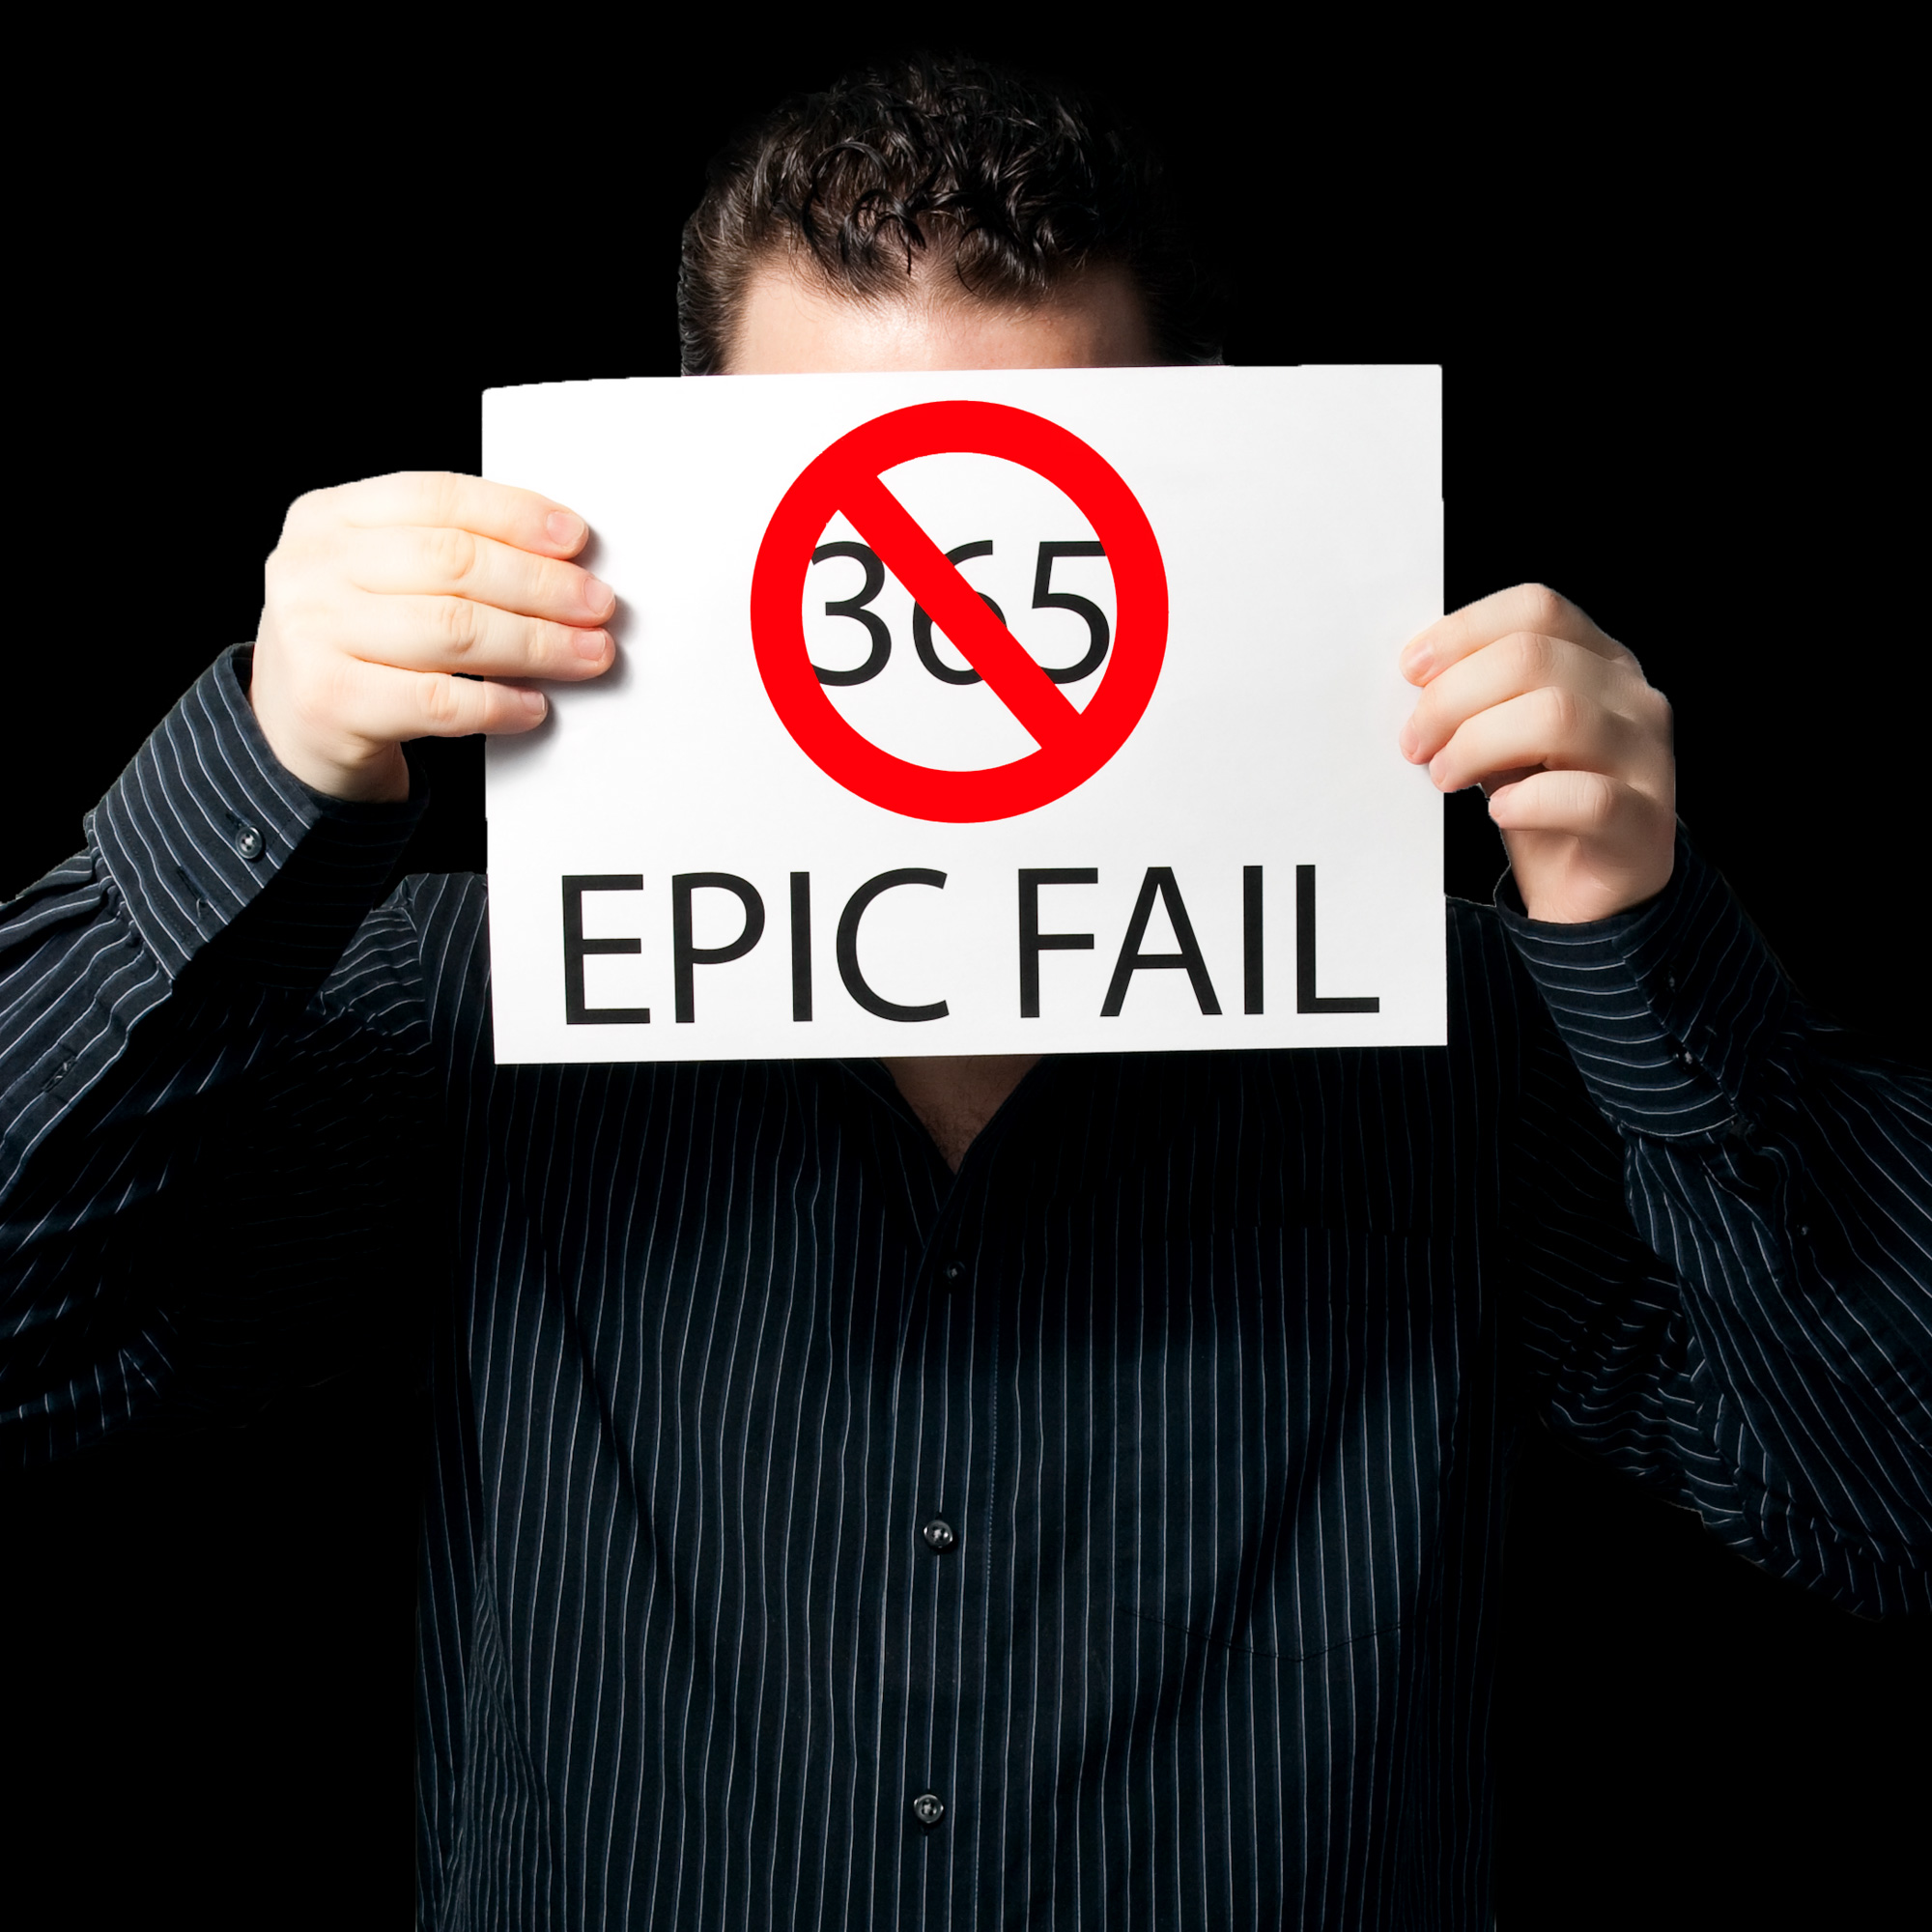
\includegraphics[width=40mm]{mittaustekniikka_pics/epicfail.jpg}

\tiny{\url{http://www.flickr.com/photos/28091490@N03/4277085203/}}

\vfill

\end{columns}

}

\frame {
\frametitle{Mitä on pielessä?}
\begin{itemize}
\item Mittaus {\bf ei ole toistokoe}. Mitattavat suureet muuttuvat.
\item Menetelmä on herkkä systemaattiselle virheelle (esimerkiksi jos mittari näyttää jatkuvasti liikaa).
\item Ohmin lain pätevyyttä ei testata, vaan se oletetaan päteväksi.
\item {Mittaustarkkuutta ei oteta huomioon ollenkaan!}
\end{itemize}
 }

\frame {
\frametitle{Oikea tapa}
\begin{itemize}
\item Selvitetään mittalaitteiden virheet (tässä esimerkissä olkoot 0,4 V ja 0,01 A).
\item Merkitään mittapisteet millimetripaperille\footnote{Esimerkiksi \url{http://www.csun.edu/science/ref/measurement/data/graphpaper/mm.pdf}}.
\item Pyri käyttämään koko millimetripaperi hyväksesi eli valitse asteikot järkevästi.
\item Piirretään mahdollisimman hyvin pisteiden kautta kulkeva suora.
\item Piirretään virhesuorat eli rajat sille, kuinka loiva tai jyrkkä suora voi pahimmillaan olla.
\item Lasketaan resistanssi suoran kulmakertoimesta.
\item Lasketaan virhearvio resistanssille virhesuorien kulmakertoimien keskiarvona.
\end{itemize}
 }

\frame {
\frametitle{Kirjallisuutta}
\begin{itemize}
\item Standardi SFS 3700\footnote{Standardi on kumottu ja korvattu käsikirjalla SFS-OPAS 99. Ei olennaisia muutoksia.}: Metrologia. Perus- ja yleistermien sanasto.
\item Pekka Wallin: Sähkömittaustekniikan perusteet. 6. painos. Helsinki 2001.
\item Pietiläinen, Merimaa: Mittaustekniikan perusteiden laboratoriotyöt. 7. korjattu painos. Helsinki 2000.
\item Kalle Ojanen: Virhelaskennan alkeita. \url{http://www.physics.utu.fi/opiskelu/opiskelijaksi/tyokurssi/index/Virhelaskkokonaan.pdf} Viitattu 31.3.2011.
\item TKK: Mittaustulosten käsittely: \url{http://tfy.tkk.fi/kurssit/Tfy-3.15x/Teoria/Tulostenkasittely.pdf} Viitattu 31.3.2011.
\end{itemize}
 }
